\section{Approach} 
\label{sec:app}
%\subsection{Overview} 
\begin{figure}[htbp] %  figure placement: here, top, bottom, or page
   \centering
   \includegraphics[width=17cm]{images/Architecture3.pdf} 
   \caption{Component view of the Architecture}
   \label{fig:SysArc}
\end{figure}

Figure~\ref{fig:SysArc} shows the component view of our proposed system architecture. It is similar to the one proposed in \cite{1}.
It is divided into two parts: An \textit{Environment Model} which stores the information about the environment and a \textit{Navigation Planning System} 
which uses the environment information to generate navigation plans.
They are both indicated by grey color blocks in the Figure~\ref{fig:SysArc}. The dotted boxes are assumed to be existing/working in the system. 
The \textit{Navigation Planning System} is further divided into three components: Semantic Navigation Planner, Navigation Knowledge base and Navigation Failure Diagnosis.
The sections below explain both parts of our architecture in detail starting with the \textit{Environment Model} and then the \textit{Semantic Navigation Planner}.\\

We consider the home environment setup of scenario 2 mentioned in section~\ref{sec:har} for explaining the architecture. 
It is assumed that the present location of the robot is \textit{livingroom-1} and it gets the goal of ``go to kitchen" from the symbolic(task) planner.  

%\input{EnvironmentModel}
%\subsection{Semantic positions}
\label{sec:semanticposition}
\subsubsection{Representing Semantic positions}
This work represents semantic positions associated with regions by three properties namely:
  \begin{itemize}
    \item \textit{Location}
    \item \textit{Orientation} 
    \item \textit{Tolerance} 
  \end{itemize}
\textit{Location} and \textit{Orientation} concepts are adopted from the approach in \cite{1}, while the \textit{Tolerance} concept is the contribution of this work.
The \textit{Location} and \textit{Orientation} properties are concerned with the x-y co-ordinate of the robot and its rotation angle with respect to local reference frame of that region.
The \textit{Tolerance} property determines how close the robot is expected to go to the semantic position.\\

These properties are represented by symbols and not by numerical values \cite{1}.
The instances of symbols for \textit{Location, Orientation} and \textit{Tolerance} properties used in this work are mentioned below:
\begin{itemize}
  \item \textit{Location} of SP: center/east/west/north/south/north-east/north-west/south-east/south-west
  \item \textit{Orientation} of SP: east/west/north/south
  \item \textit{Tolerance} for SP: soft/medium/hard
\end{itemize}
An example of a semantic position for \textit{kitchen-1} instance of our home environment setup is shown below:
\begin{itemize}
  \item \textit{Location}: center
  \item \textit{Orientation}: north
  \item \textit{Tolerance}: soft/medium/hard
\end{itemize}
The definitions/equations of these symbols are stored in the \textit{Navigation Equations component} of the architecture elaborated in section~\ref{sec:ne} .
However, depending on the application domain, the symbols could be added/removed/modified along with their definitions in the \textit{Navigation Equations component}.\\

Usually rooms and other categories of \textit{Region} concept will have soft or medium tolerance.
\textit{Objects} will mostly have hard tolerance.
These assumptions may change depending on the application domain.

\subsubsection{Advantage of \textit{Tolerance} limit} 
\textit{Tolerance} limit for a semantic position makes navigation flexible in the following way:
Usually a robot goes to a room and then proceeds towards some object.
For instance, in our home environment setup, suppose the robot is given the task of ``bringing a milk bottle". The robot needs to go to the
kitchen and dock a fridge to pick-up the milk bottle. In such scenarios, the robot does not need to reach the exact semantic position of the kitchen.
%it is acceptable if the robot does not exactly reach the kitchen's semantic 
%position since there its is not expected to manipulate any object. Instead it has to approach the fridge after entering the kitchen. 
Assigning soft tolerance to the semantic position of the kitchen enables the robot to conclude the accomplishment
of the goal of ``going to kitchen"  as soon as it is in the kitchen.\\

For the same task, after reaching the kitchen the robot has to dock the fridge to grasp a milk bottle. Hence, fridge could have medium tolerance limit indicating
that robot has go near to the fridge. This nearness depends on the workspace of the robot platform. A hard tolerance limit indicates that the robot has to be at the exact position.
Assigning a hard or soft tolerance limit to the semantic position of an object depends on the workspace of the robot. Robots with limited workspace need to
have hard tolerance to grasp objects. However, regions can always have a soft tolerance limit, irrespective of the platform workspace,
unless robots are not grasping any objects at those positions.\\

The tolerance limit helps to deal with situations in which dynamic obstacles in the vicinity or on the semantic positions. 
It also improves the path planning efficiency by reducing the goal completion time.
%\subsection{Navigation Planning System}
\begin{figure}[htbp] %  figure placement: here, top, bottom, or page
 \centering
   %\includegraphics[angle=90,width=10cm]{images/tbox.jpg}
   \includegraphics[width=23.6cm, height=13cm, angle=90]{images/snp_1backup.pdf}
   \caption{Navigation Planning System}
   \label{Fig: Method of storing geometric shape of the room}
\end{figure}
We consider an example in the home environment setup of scenario 2 mentioned in section~\ref{sec:har}  for explaining the system. 
In this example, the robot gets a symbolic goal of ``go to kitchen" from the high 
(task/symbolic) level planner. Let us assume the current semantic location of the robot 
as ``living room".

\subsubsection{Overview}
The system works in three stages:
\begin{itemize}
 \item Planning: At this stage the navigation is planned by dividing the symbolic goal received from the high level (task) planner into an array of geometric sub-goals.
 \item Monitoring: This stage feeds the geometric sub-goals to the motion planner and monitors its execution.
 \item Recovery: This stage is initiated if the robot is not able to achieve its goal/sub-goal. At first the cause of failure is identified and then the necessary recovery is conducted.
\end{itemize}

The \textit{Navigation Planning System} gets its goal ``go to kitchen" from the high level 
(task / symbolic) planner.
The \textit{Environment model} is then queried about the robot's current semantic position which in this case is the \textit{living room-1}.
Accordingly, the system generates a semantic navigation plan consisting of a set of sequential symbolic sub-Version1goals.
In this example, the semantic navigation plan is: ``go to \textit{doorway-1}", ``go to \textit{kitchen-1}".
Once this abstract plan is generated, the planner system queries the \textit{model} again, this time asking for corresponding semantic positions associated with these region instances (\textit{doorway-1, kitchen-1}).
These semantic positions are then fed to the motion(path) planner in a sequence.
If the robot is not able to reach its goal/sub-goal (\textit{kitchen-1}), the planning system searches for the cause (may be blockage of \textit{doorway-1} due to malfunctioning of \textit{door-1})
and accordingly modifies the plan to achieve the goal.
If the goal is not achieved even after executing all possible/relevant recovery options, the planner sends a failure notification along with the cause
to the high level planner.\\

Sections below explain working of each component of our proposed system. Figure~\ref{fig:legend} gives the meaning of the symbols used to explain component.
\begin{figure}[htbp] %  figure placement: here, top, bottom, or page
   \centering
   %\includegraphics[angle=90,width=10cm]{images/tbox.jpg}
   \includegraphics[width=6cm]{images/snp_legend.pdf}
   \caption{Legend for Navigation Planning System of Figure~\ref{Fig: Method of storing geometric shape of the room}}
   \label{fig:legend}
\end{figure}

\subsubsection{Plan Generator}
\begin{figure}[htbp] %  figure placement: here, top, bottom, or page
   \centering
   %\includegraphics[angle=90,width=10cm]{images/tbox.jpg}
   \includegraphics[width=12cm]{images/snp1_1.pdf}
   \caption{Plan Generator component}
   \label{Fig:Data flow summery}
\end{figure}
This is the component where actual navigation plans are generated for the motion(path) planner.
It gets a symbolic navigation goal from a high level (task/symbolic) planner, for instance, ``go to \textit{kitchen-1}".
Once it gets a goal, it queries the \textit{Localization cache} about robot's current semantic position (\textit{living room-1} in our example).
Then it queries the \textit{Environment Model} via the \textit{Map cache} component to get the topological connectivity between 
the robot's current semantic position(\textit{living room-1}) and the semantic goal(\textit{kitchen-1}).
This symbolic goal is then divided into symbolic sub-goals (``go to \textit{doorway-1}", ``go to \textit{kitchen-1}") based on the response 
from the \textit{Environment Model}.
Further, the semantic positions of these subgoals are queried(to the \textit{Environment Model} via the \textit{Map cache}) and a sequence of geometric sub-goals i.e semantic positions with constraints, is generated. 
Each sub-goal has a set of constraints which could be geometric, kinematic, dynamic or semantic. 
This work considers only semantic and dynamic constraints.
Semantic constraints include tolerance limit associated with each semantic position.
For dynamic constraints we consider robot velocity and acceleration.
Once a set of sequential (geometric) sub-goals with constraints is generated, it is fed to the next component, that is, the \textit{Scheduler}.  

\subsubsection{Scheduler}
\begin{figure}[htbp] %  figure placement: here, top, bottom, or page
   \centering
   %\includegraphics[angle=90,width=10cm]{images/tbox.jpg}
   \includegraphics[width=5cm]{images/snp2.pdf}
   \caption{Scheduler component}
   \label{Fig:Data flow summery}
\end{figure}
The \textit{Scheduler} component is a data base which maintains the sub-goals in a sequential manner as generated by \textit{Plan Generator} component.
It also stores the associated constraints for each sub-goal as shown in the Figure ~\ref{fig:s} .
In our example, sub-goal $g_{1}$ is the semantic position associated with \textit{doorway-1} and $g_{2}$ is semantic position for \textit{kitchen-1}.
$c_{1}, c_{2}$ as indicated in the figure are the constraints: {tolerance limit, velocity, acceleration}. 
Each sub goal is fed to the motion(path) planner through the \textit{Monitor Unit}, upon receiving the previous goal completion notification. 
For instance, once the sub-goal $g_{1}$ is fed to the motion(path) planner (through the \textit{Monitoring} component), the \textit{Scheduler} will wait for a response from 
the \textit{Monitoring} component about completion of sub goal $g_{1}$ before sending the next sub goal $g_{2}$.

 \begin{figure}[htbp]
 \centering
 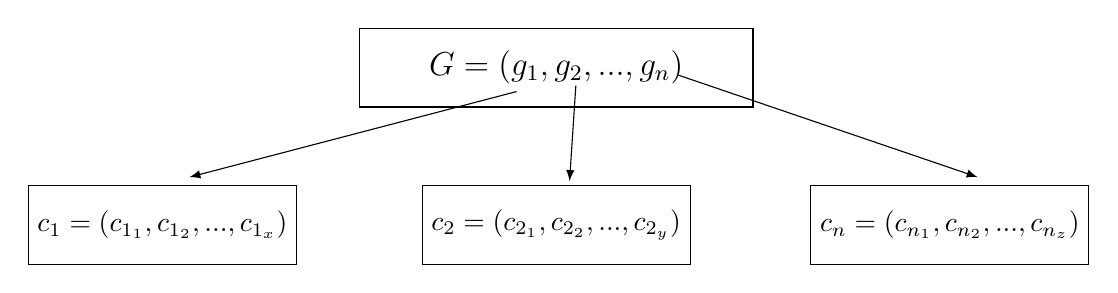
\begin{tikzpicture}
% two boxes
\node[draw,minimum width=5cm, minimum height=1cm] (a) at (5,0) {\large $G = (g_{1} ,  g_{2} ,...,  g_{n})$};
\node[draw,minimum width=3cm, minimum height=1cm] (b) at (0,-2) {$c_{1} = (c_{1_1},c_{1_2},...,c_{1_x})$};
\node[draw,minimum width=3cm, minimum height=1cm] (c) at (5,-2) {$c_{2} = (c_{2_1},c_{2_2},...,c_{2_y})$};
\node[draw,minimum width=3cm, minimum height=1cm] (d) at (10,-2) {$c_{n} = (c_{n_1},c_{n_2},...,c_{n_z})$};

\path (a.east) -- (a.south west) coordinate[pos=0.6] (a1);
\path (b.west) -- (b.north) coordinate[pos=1.2] (b1);
\draw[latex-] (b1) -- (a1);

\path (a.east) -- (a.south west) coordinate[pos=0.45] (a2);
\path (c.west) -- (c.north) coordinate[pos=1.1] (b2);
\draw[latex-] (b2) -- (a2);

\path (a.east)  -- (a.south west) coordinate[pos=0.19] (a3);
\path (d.west) -- (d.north) coordinate[pos=1.2] (b3);
\draw[latex-] (b3) -- (a3);
\end{tikzpicture}
 \caption[Symbolic goal, geometric subgoals and constraint lists]
 {G is the symbolic goal which is segmented into geometric subgoals of $g_{1},...,g_{n}. c_{1}...c_{n}$ represents associated list of constraints}
 \label{fig:s}
\end{figure}

\subsubsection{Monitoring}
\begin{figure}[htbp] %  figure placement: here, top, bottom, or page
   \centering
   %\includegraphics[angle=90,width=10cm]{images/tbox.jpg}
   \includegraphics[width=12cm]{images/snp3.pdf}
   \caption{Monitoring component}
   \label{Fig:Data flow summery}
\end{figure}

The purpose of this component is twofold:
  \begin{itemize}
   \item The \textit{Monitoring} component acts as a coordinator between the \textit{Scheduler} and the motion(path) planner.
   \item Monitoring the working of the motion planner while it attempts to reach the given goal/sub goal.
\end{itemize}
The \textit{Monitoring} component queries the \textit{Scheduler} for a subgoal(with constraints) and 
sends it to the motion planner depending on its status(whether the planner is free).
It then monitors the motion(path) planner executing the given subgoal.
The motion planner notifies the \textit{Monitoring} component about the completion of the sub goal by firing an event.
The motion planner triggers a failure event if the previous sub goal is not achieved, notifying the \textit{Monitoring} component about the failure.
In situations of failure the \textit{Monitoring} component informs the \textit{Navigation Failure Diagnosis} unit.\\

Another important function the \textit{Monitoring} component is expected to perform is setting appropriate parameters\footnote[6]{ROS Navigation stack consist of a set of parameters for (global and local) planners which could be set to customize the behavior of the planners. \url{http://wiki.ros.org/navigation/Tutorials/RobotSetup}. [Online]. Accessed: Oct. 22, 2013] } 
for the motion planner to satisfy the given constraints. 
However, this might not be necessary for some constraints.
For instance, in our work the tolerance limit constraint associated with semantic positions has a different role to play.
It is used for the purpose of monitoring and helps in deciding when to conclude that the given subgoal is achieved.
Hence, the constraint of tolerance limit is not set by the \textit{Monitoring} component.

\subsubsection{Navigation Equations}
\label{sec:ne}
\begin{figure}[htbp]
 \centering
 \includegraphics[width=8.5cm]{images/snp4.pdf}
 \caption{Navigation Equation component}
 \label{Fig:Data flow summery}
\end{figure}

As the name suggests, \textit{Navigation Equations} component contains a set of equations(rules) which can perform certain calculations \cite{1,21}.
The calculations are performed on the properties of the \textit{semantic positions}, that is on \textit{Location, Orientation} and \textit{Tolerance}
properties which have symbolic values.
Example: \textit{Tolerance} can have symbolic values such as \textit{soft/medium/hard}.
These symbolic values are fed as input to the \textit{Navigation Equations} component which performs calculations on them
to convert them into appropriate numerical values.
For instance, if semantic position of \textit{kitchen-1} has a symbolic value \textit{center} for \textit{Location}, then 
these values are fed to the \textit{Navigation Equations} component. 
The component returns a numerical value for the symbolic value \textit{center} using the equation mentioned below:\\

\begin{center}
\begin{Large}
$ x_{center} = \frac{ w_{l} + x + w_{r} }{2}$
 
$y_{center} = \frac{ h_{l} + h + h_{r} }{2}$
\end{Large}
\end{center}

 \begin{figure}[htbp]
 \begin{center}
 \includegraphics[width=10cm]{images/geometry.png}
 \caption[Navigation equation example(up). Region geometry(down) represented by triple \cite{8}]
 {Navigation equation example(up). Region geometry(down) represented by triple $G_{R}$=\textit{(x, y, w, h, $\theta$, $w_{l}$, $h_{l}$, $y_{l}$, $w_{r}$, $h_{r}$, $y_{r}$)} \cite{8}} 
\label{Fig:Data flow summery}
\end{center}
\end{figure}

Similar equations exist for other symbolic values of \textit{Location} and for other properties of semantic positions.
These symbolic values and their definitions could be changed depending on the domain. 
Maintaining equations in a separate component helps to reduce the complexity of the system by decreasing the number of facts to be stored explicitly in the map \cite{1}.
\subsubsection{Map cache}
\begin{figure}[htbp]
 \centering
 \includegraphics[width=12cm]{images/snp5.pdf}
 \caption{Map cache component}
 \label{Fig:Data flow summery}
\end{figure}

The \textit{Map cache} temporarily maintains the environment information relevant for the navigation task being executed.
For instance, in our example, the \textit{Map cache} component maintains occupancy grid maps of \textit{livingroom-1, doorway-1, kitchen-1} along with their topological connectivity.
It also maintains their semantic positions.
Other units like the \textit{Semantic Navigation planner} or \textit{Navigation Failure Diagnosis}  query the \textit{Map cache} 
component for environment information. 
For the first time, the \textit{Map cache} queries the \textit{Environment Model} about environment information, after receiving a request about it from the \textit{Navigation planner} component.\\
This information is then maintained by the \textit{Map cache} either until the symbolic goal is achieved or till a new request is generated by the \textit{Navigation planner} component.
If some additional information is required while execution, for instance by the \textit{Navigation Failure Diagnosis} unit while dealing with unexpected situations(failures), 
it is queried to the \textit{Environment model} via the \textit{Map cache} component.

\subsubsection{Localization cache}
\begin{figure}[htbp]
 \centering
 \includegraphics[width=12cm]{images/snp6.pdf}
 \caption{Localization cache component}
 \label{Fig:Data flow summery}
\end{figure}

The \textit{Localization cache} component maintains a constant update of the robot's current location 
(semantic+topological+metric).
It gets its input from the on-line SLAM algorithm.
%Based on this it will calculate the average probability of location.
The \textit{Monitoring} and other components query the\textit{ Localization cache} for the robot's current semantic location.

\subsubsection{Navigation Failure Diagnosis(\textit{Reasoning and Recovery})}
\begin{figure}[htbp]
 \centering
 \includegraphics[width=12cm]{images/snp7.pdf}
 \caption{Navigation Failure Diagnosis Unit}
 \label{Fig:Data flow summery}
\end{figure}
During the execution of the given sub-goal, if there is a failure,
it is notified to the \textit{Navigation Failure Diagnosis} unit by the \textit{Monitoring} component by triggering a failure event.
The \textit{Navigation Failure Diagnosis} unit then takes control over the low level planners\footnote[7]{Low level planners include the global planner at the motion planning level and the local planner at the controller level as shown in Figure~\ref{fig:SysArc}} 
to overcome the situation.
While the \textit{Navigation Failure Diagnosis} unit is trying to overcome the unexpected situation, it notifies the \textit{Monitoring }component to wait until the recovery is done.
If no solution works for recovering from the situation, the high level (task/symbolic) planner is notified about the symbolic goal failure. \\

However, Failure Diagnosis and Reasoning in robotics are vast fields and under active research.
Hence in this work, we consider Failure Diagnosis for navigation at a naive level. The \textit{Navigation Failure Diagnosis} unit 
needs thorough research and evaluation which is out of the scope of this work.
Our \textit{Recovery} component consists of a set of recovery behaviors which are initiated to recover from unexpected situations.
For instance, one of the recover behaviors our \textit{Recovery} component has is the rotate recovery behavior\footnote[8]{The current ROS Navigation Stack has such a rotate recovery behavior. 
Details of this can be found on: \url{http://wiki.ros.org/rotate_recovery}}.\\

\iffalse 
\subsection{Significance of adding semantic positions for \textit{Regions} and \textit{Objects}:}
\begin{itemize}
  \item In this work, to begin with, our semantic positions will be represented by three properties, namely:
  \begin{itemize}
    \item Location of SP: center/east/west/north/south/north-east/north-west/south-east/southth-west
    \item Orientation of SP: east/west/north/south
    \item Tolerance for the SP: soft/medium/hard
  \end{itemize}
  \item The location and orientation properties are concerned with the x-y co-ordinate (location) of the robot and its rotation angle (orientation) at that location.
  \item The tolerance property is of importance here for navigation.
  \item It determines how close the robot is expected to go to the semantic position.
  \item Usually rooms and other categories of region concept will have soft or medium tolerance.
  \item Objects will mostly have hard tolerance.
  \item However, these assumtions may cahnge depending on the application domain.
  \item This property will be helpful for navigation in the following way:
  \item Usually a robot has to go to any room and has to navigate towards some object.
  For example, for a home assistant robot, it has to go to the kitchen and dock a fridge to pick-up a milk bottle, or dock to the dinner table for cleaning it, or dock to a oven and so on.
  \item For all such situations it is acceptable if the robot does not eaxctly reach the kitchen's semantic position since it has to go to other position (semantic position fo the object to be manipulated).
  \item This will help to deal with situations such as if a person or other obstacle is standing on the semantic position of the room.
  \item Also it might save cost, since one the robot is in the room it can start executing its next path plan. \\\\\\\\
      
    
    \item Location: Indicate the location on x-y plane.
    \item However, in this approach we make use of concepts instead of numerical values to indicate the location.
    \item The location concept will have following instances: center, east, west, north, south.
    \item We can have additional/different instances of the concept location depending on the needs of the domain.
    \item Orientation: The orientation concept will have following four instances: north, south, east, west.
    \item Tolerance: The tolerance concept will have three instances: soft, medium an hard.
    \item soft tolerance will usually be assigne to semantic positions belonging to Region instances.
    \item For instance suppose robot is approaching the kitchen,that is to the semantic position(tolerance: soft) of kitchen. 
    \item soft tolerance will indicate the navigation planning system that it is not required for the robot to be exactly(in terms of x,y cordinates and orientation) at the semantic position.
    \item Instead, the navigation system can conclude that the goal(sub-goal) is achieved as soon as its localization unit etects that the robot has reached the kitchen.
    \item We believe this will help the navigation system to be flexible and help to deal with unexpected situations. Details of the same areexplained in next section.
    \item The locationa dn orientation concepts are adopted from the approach in \cite{8}.
    \item However, adding tolerances to the semantic positions is the contribution of this work.
  
\end{itemize}
\fi
%\subsection{Case Study}
\subsubsection{Home environment for personal assistant robot}
\begin{figure}[htbp] %  figure placement: here, top, bottom, or page
   \centering
   %\includegraphics[angle=90,width=10cm]{images/tbox.jpg}
   \includegraphics[width=12cm]{images/example.pdf}
   \caption{Home environment setup}
   \label{Test environment map}
\end{figure}
In this section with the help of an example we explain the working of our proposed system.
Considering the home environment setup mentioned in section~\ref{sec:har} the robot is given the goal of ``go to kitchen".
The current semantic location of the robot is taken to be \textit{livingroom-1}.
Thus the robot has to start from \textit{livingroom-1} and go to \textit{kitchen-1}.\\

Our proposed \textit{Navigation Planner System} works as elaborated below:\\ 
First, the \textit{Semantic Navigation Planner} unit receives the goal ``go to \textit{kitchen-1}" from the high level (task/symbolic) planner.
Then it queries the \textit{Environment Model} about the topological connectivity between the two \textit{Region} instances.
In this example the two regions are connected as follows:
\textit{livingroom-1} $\longleftrightarrow$ \textit{doorway-2} $\longleftrightarrow$ \textit{kitchen-1}\\
The \textit{Semantic Navigation Planner} unit then queries the \textit{Environment Model} for corresponding semantic positions for each of the above region instances.
Thus, the symbolic goal of ``go to the kitchen" is converted to geometric sub-goals: \textit{go to SP2}, \textit{go to SP3}, where \textit{SP2} represents semantic position for Doorway-2 and \textit{SP3} for Kitchen-1.
These sub-goals along with associated constraints are stored in the \textit{Scheduler} component of the \textit{Semantic Navigation Planner} unit .
It is assumed that \textit{SP2} has a medium tolerance and \textit{SP3} has a soft tolerance and the other semantic properties and constraints are neglected.
Each of these sub goals is then fed to the \textit{Monitoring} component which further passes it to the motion planner.
Once the sub goal \textit{SP3} is achieved, the motion planner triggers an event, notifying the completion of the sub goal to the \textit{Monitoring} component.
After receiving this notification the \textit{Monitoring} component feeds the next sub goal and this continues till the last sub goal is achieved.\\

\textbf{Dealing with unexpected situations:}\\
\textit{Situation 1:}\\
Suppose the robot is not able to reach \textit{SP2}.
The motion(path) planner notifies the \textit{Monitoring} component about this failure by triggering a failure event.
The \textit{Monitoring} component then notifies the \textit{Navigation Failure Analyzer} about this goal/sub goal failure.
To identify the cause of failure the \textit{Navigation Failure Analyzer} queries the \textit{Environment Model} for current environment and robot's state.
We assume \textit{doorway-2} has a automatic \textit{door-2} since in this work we consider doorways with only automatic doors.
Based on this information, the \textit{Failure Analyzer}  concludes the cause of failure as malfunctioning of \textit{door-2} at \textit{doorway-2} (assuming the \textit{Failure Analyzer} is capable of detecting such failures).
Since in such situations it is not possible to navigate through \textit{doorway-2}, the \textit{Navigation Failure Analyzer}
notifies the high level planner about the goal failure.\\

\textit{Situation 2:}\\
To demonstrate the flexibility provided by the tolerance limit we consider the situation where the goal \textit{SP2} is achieved and the robot is now approaching \textit{SP3}.
Since \textit{SP3} has \textit{soft} tolerance limit, the planner concludes the sub goal to be achieved as soon as the robot is in the kitchen.
This proves to be helpful in situations where there is a dynamic obstacle on or in the close vicinity of the semantic position.

%\subsubsection{Case 2: University environment for library assistant robot}

In this section we will briefly describe the approach taken to propose a solution model for the problem formulation. Then we go on to propose an experimental setup which will validate the proposed method.

%of the approach is to implement the lawnmower algorithm
\subsection{Overview}

A scientific approach to any problem, requires an extensive research on the state of the art that exists for this particular problem, which has already been done in the previous section. 
The first step is to determine on what factors does the performance of the back and forth or lawnmower method -suggested in  \cite{1,2,3,8,10}- depend on, and record those parameters:
\begin{itemize}
\item Time of coverage
\item Trace of the UAV's path
\item Velocity - both linear and angular
\end{itemize}
The next step is to determine algorithms which will minimize these parameters. From \cite{6} we learned that using simple trajectories like hemispherical - see figure ~\ref{fig:hchc} - and cylindrical - see figure ~\ref{fig:cchc} - we can do coverage of any area. After implementing the algorithms which will be formulated in ~\ref{subsec:fml343}, the next step will be to record the above mentioned parameters and compare with the lawnmower approach parameters. 

\subsection{Formulating mathematical model of the algorithms}
\label{subsec:fml343}
In \cite{6} the authors propose hemispherical - see figure ~\ref{fig:hchc} - and cylindrical trajectories - see figure ~\ref{fig:cchc} - for 3D coverage, likewise for 2D coverage we can use smooth curves like spirals, splines and Lissajous Curves to generate trajectory path for the UAVs. In this section we will describe the mathematical models of the above mentioned curves.
\subsubsection{Spiral}
\textbf{Spiral} - According to the The American Heritage Dictionary of the English\footnote{The American Heritage Dictionary of the English Language, Houghton Mifflin Company, Fourth Edition, 2009.} a spiral is defined as a curve which winds around a fixed center point at continuously increasing or decreasing radius. 
\footnotetext{http://www.mathematische-basteleien.de/spiral.htm}
For generating way-points we need to use the parametric equation of a spiral, given by\footnotemark \\ 
\begin{equation}
\label{eq:sp1}
x(t) = at cos(t)
\end{equation}
\begin{equation}
\label{eq:sp2}
y(t) = at sin(t)
\end{equation}

In ~\ref{eq:sp1}, ~\ref{eq:sp2} $x$ and $y$ are the coordinates of the waypoints, $a$ is a constant value and $t$ is the varying radius.
The value of $a$ will depend on the dimensions of the maximum value of $x$ and $y$. The parameter $t$ can be adjusted to increase or decrease the width between two successive curves of the spiral. This value will be adjusted according to the field of view radius of the UAV sensor.

\begin{figure}[htbp] %  figure placement: here, top, bottom, or page
 \centering
   %\includegraphics[angle=90,width=10cm]{images/tbox.jpg}
   \includegraphics[width=9cm]{images/coverage_12.png}
   \caption[Archimedean Spiral ]
   {Archimedean Spiral \footnotemark[\value{footnote}]}
   
\label{fig:sc111}
\end{figure}

\subsubsection{Lissajous Curves}
\textbf{Lissajous Curves} - From the work in \cite{14} we get the parametric for of Lissajous curves. \\
\begin{equation}
\label{eq:ls1}
x(t) = Acos(\omega_xt-\delta_x)
\end{equation}
\begin{equation}
\label{eq:ls2}
y(t) = Bcos(\omega_yt-\delta_y)
\end{equation}
\begin{equation}
\label{eq:ls3}
x(t) = Asin(\omega'*t+\delta)
\end{equation}
\begin{equation}
\label{eq:ls4}
y(t) = Bsin(\omega*t)
\end{equation}
In equations ~\ref{eq:ls1},~\ref{eq:ls2},~\ref{eq:ls3},~\ref{eq:ls4} $x$ and $y$ are the coordinates of the waypoints, $\omega_xt$ and $\omega_yt$ are the amplitude of the $cosine$ curve, $\omega'$ and $\omega$ are the amplitudes of the $sine$ curve and $\delta$, $\delta_x$ ,$\delta_y$ are the necessary phase difference to create a Lissajous pattern and $t$ is a variable. 
If the ratio of $\frac{\omega'}{\omega} = 5/4$, the following Lissajous pattern can be generated - see figure: ~\ref{fig:ljc221} -  which can act as a space filling curve, thus in our case act as an algorithm for coverage.

\begin{figure}[htbp] %  figure placement: here, top, bottom, or page
 \centering
   %\includegraphics[angle=90,width=10cm]{images/tbox.jpg}
   \includegraphics[width=9cm]{images/coverage_11.png}
   \caption[Lissajous Curve \cite{14}]
   {Lissajous Curve with $\frac{\omega'}{\omega} = 5:4$  \cite{14}}
   
\label{fig:ljc221}
\end{figure}

\subsubsection{Hybrid of Spiral and Lissajous Curves}
To generate this Lissajous Curve ~\ref{fig:hsjc3333}, the ratio of $\frac{\omega'}{\omega}$ was set to $1:2$, while varying the value of $t$(in this case increasing) with each iteration we create the following coverage pattern. This pattern can be used in case of doing coverage while persistently tracking any target object. The center of the curve where the spirals intersect can be fixed on a target object and the UAV can cover an area while persistently tracking the target object.

\begin{figure}[htbp] %  figure placement: here, top, bottom, or page
 \centering
   %\includegraphics[angle=90,width=10cm]{images/tbox.jpg}
   \includegraphics[width=9cm]{images/coverage_14.png}
   \caption[Lissajous Curve \cite{14}]
   {Hybrid approach based on Spiral and Lissajous Curves method  \cite{14}}
   
\label{fig:hsjc3333}
\end{figure}

\pagebreak
\subsubsection{Rapidly Exploring Random Trees}
Along with the above mentioned geometrical approaches we also implement a randomized approach in order to have a better comparison of our proposed method. Unlike probabilistic approaches which require point to point convergence to progress \cite{15}, we require an approach which can randomly expand and fill a coverage space. Rapidly Exploring Random Trees are thus ideal for our problem\cite{15}. The only change we make here is that we do not consider a shortest path between start and goal node, instead we try to generate a large number of nodes in the space to be covered and use these generated nodes as waypoints for the UAVs to follow. We try to order the waypoints generated in ascending order of Euclidean distance from the starting point.

\begin{figure}[htbp] %  figure placement: here, top, bottom, or page
 \centering
   %\includegraphics[angle=90,width=10cm]{images/tbox.jpg}
   \includegraphics[width=9cm]{images/coverage_13.png}
   \caption[Rapidly Exploring Random Tree \cite{15}]
   {Rapidly Exploring Random Tree \cite{15}}
   
\label{fig:rrt}
\end{figure}

\subsection{Performance Metric Function}

An effective means of comparing methods, which are dependent on multiple parameters is to formulate a performance metric function with certain weights assigned to each parameter. The performance metric function will take into account percentage of area covered, percentage of overlap, percentage of area it exceeds from the commanded area, time of coverage and energy consumed during run (which depends on the rate of change of velocity during its motion). The highest weight-age will be assigned to percentage of area coverage, time required to completion, and energy cost. The parameters percentage of area overlap and percentage of area exceeded will be assigned lower weight-age value as these parameters have lower effect on the performance of the proposed algorithms.

\subsection{Experimentation}

For carrying out our experiment we will adopt the rolling landscape scenario from Gazebo simulation environment. We will consider a coverage space of certain size and vary the following parameters for each of the aforementioned algorithms - 
\begin{itemize}
\item Number of waypoints 
\item Size and shape of the area to be covered
\end{itemize}
After implementing the above mentioned algorithms using ROS and Hector Quadrotor package, we will record the ground truth information of the UAVs. 

\subsection{Evaluation}

From the experiments that will be carried out in section: ~\ref{subsec:exp2211} we will record the following values
\begin{itemize}
\item Time
\item X,Y,X poses
\item Linear X velocity, Linear Y velocity, Linear Z velocity
\item Angular X velocity, Angular Y velocity, Angular Z velocity
\end{itemize}

Next we will evaluate the implemented methods based on these parameters and determine which method is best suited for coverage in a certain space. The evaluation criteria will be explained in details in the next section. 